\documentclass[pdftex,12pt,a4paper]{article}

\usepackage[pdftex]{graphicx}
\usepackage{graphicx}
\usepackage{picture}
\usepackage{graphics}
\usepackage{amsmath} % for argmax
\usepackage{bm} % used for bolding the equation

\newcommand{\HRule}{\rule{\linewidth}{0.5mm}}
\DeclareMathOperator*{\argmin}{argmin}

\begin{document}

\begin{titlepage}

\begin{center}


% Upper part of the page

\includegraphics[width=0.15\textwidth]{./uml_logo}\\[5cm]    

\textsc{\LARGE Computer Graphics I}\\[1.5cm]

\textsc{\Large Literature Reivew III}\\[0.5cm]


% Title
\HRule \\[0.4cm]
{ \huge \bfseries Local deep feature learning framework for 3D shape}\\[0.4cm]

\HRule \\[1.5cm]

% Author and supervisor
\begin{minipage}{0.4\textwidth}
\begin{flushleft} \large
\emph{Author:}\\
Chang \textsc{Liu}
\end{flushleft}
\end{minipage}
\begin{minipage}{0.4\textwidth}
\begin{flushright} \large
\emph{Teacher:} \\
Dr.~Haim \textsc{Levkowitz}
\end{flushright}
\end{minipage}

\vfill

% Bottom of the page
{\large \today}

\end{center}

\end{titlepage}

\section{Abstract}
\indent Object recognition, human pose estimation are applications which are frequently solved through a decomposition into a collection of parts. Detection and recognition require modelling the appearance of the different object parts, and it also requires to model the spatial layout. These representation has already been shown successfully in body part estimation from depth images.

In today's top research in this area, deep learning has gradually shown its full potential, by integrating spatial layout into parts classification without costly pairwise terms during testing, the paper shows that the method classifies pixels independently with a very high precision using convolution neural network.

\section{Overview}
\indent The selected papers are ''\textbf{Human body part estimation from depth images via spatially-constrained deep learning}'' and ''\textbf{Local deep feature learning framework for 3D shape}''. The reason that I choose these two papers are that I find that deep features are a very popular topic in graphic research, how to represent the image or 3D shape well is closely in relation to the feature selection. By choosing different models and feature representation, we could get very different performance and accuracy. In these two papers, the authors both give a very detailed description about the feature selection and how it works in mathematical theory, and I find that by understanding their model, I could get a basic knowledge behind them, and may apply them to my research in the future.

\subsection{Spatially-constrained features}
\indent In the first paper, the author gives a very detailed description about how it works when spatial layout is taken into consideration for a very large dataset in the human body parts.

As in current research trend shows, the segmentation algorithm typically considers local appearance information, and frequently also models the spatial relationships between different parts. However, then considering these factors, their relationship within the segmentation process mostly amounts to solving constraint satisfaction problems. So in this paper, the author address the problem of efficient modeling spatial relationship without the need for solving complex combinatorial problems.

\subsection{Deep learning}
\indent As deep learning has multiple layers structures in different scenarios, the spatial representation is difficult to directly be shown in hard-coded features. And by using traditional representation like SIFT, HOG or other descriptor, it seems that deep features is a better way to adapt to the complex images. So in this paper, they apply the deep learning algorithm to this field, and it really works well according to their result.

In their experiment, the architecture for deep learning is convolutional neural network, here they use a simple structure for the deep learning,for the detailed construction of the network, please refer to the following figure:

\begin{center} % add this to make the figure shows in the middle of the pages
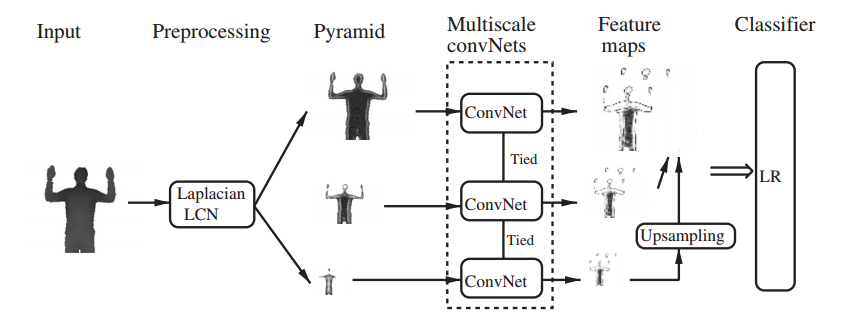
\includegraphics[scale=0.4]{lit-rev3-2.png}
%\caption{EHD descriptor for distinguishing the image}
\end{center}

From the above figure, it shows that it contains preprocessing, pyramid, multiscale convNets, feature maps and classifier. In this multiscale convNets, different convNets are connected by their ties between them. Since many visual recognition problems require a large context due to complex interaction.

For the training of this deep learning architecture, it contains two steps. The first step is the spatial deep learning layout. And
it is also called weakly supervised pre-training. At this stage, the ConvNet parameters are initialized such that the features are consistent with the spatial arrangement of the labels. The second step is supervised spatial learning. A logistic regression layer parameterized with $h_{g}$ is connected to the topmost feature maps of the ConvNet to predict the labels. They also apply a fine-tuning scheme in which the gradients from the $LR$(Logistic Regression) are back-propagated to update the the ConvNet parameters $h_{f}$.


\subsection{3D-shape in deep learning}
After the discussion of the first paper, we should know that deep learning is quite a good representation of a image segmentation. And in other areas like 3D-object detection, it also has a wide range of application in these field. 3D-shape could be considered as a complex multi-dimensional formation of the images, and it also should gives a structure of the neural network.

For 3D-shape analysis, the second paper uses four steps to address this issue. 

1)First, several basic descriptors are calculated to generate bag-of-words to use the various basic descriptor's properties.

2)3D mesh is down-sampled to hundreds of feature points for accelerating the model learning. 

3)Then, encode the bag-of-words into local geodesicaware bag-of-features (LGA-BoF). 

4)At last, use deep belief networks (DBNs) to learn a model, and use it to generate the LDF for 3D-shapes.

The detailed figure is shown as below:

\begin{center}
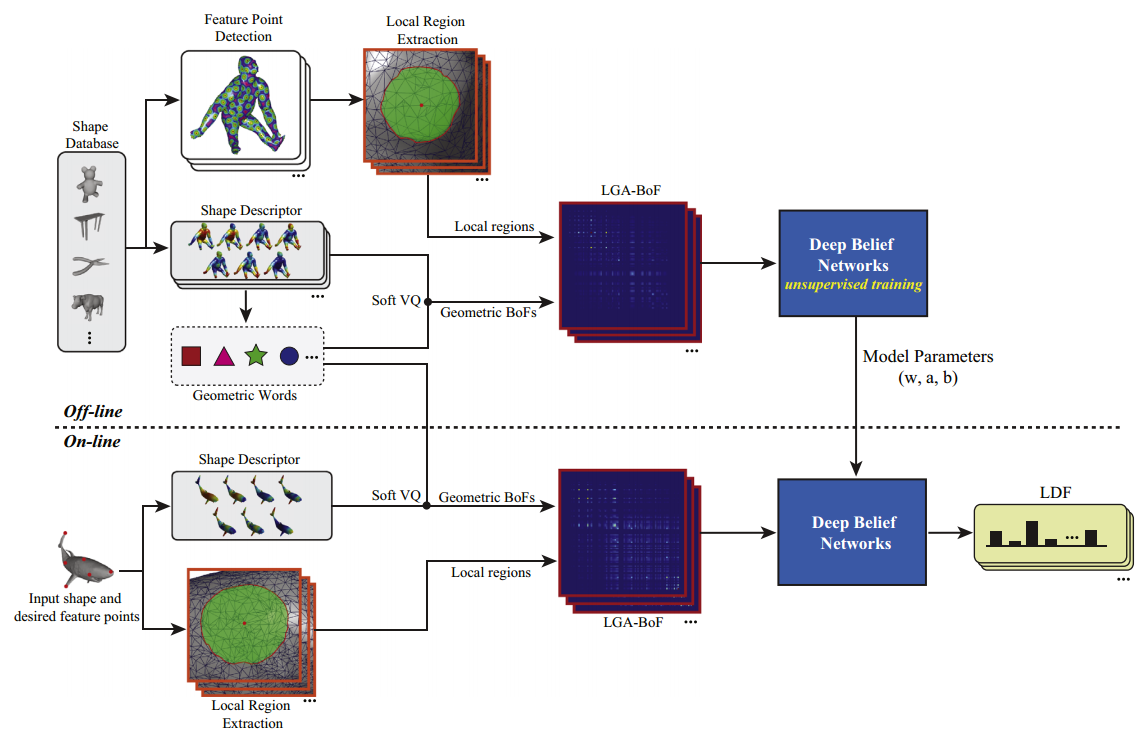
\includegraphics[scale=0.3]{lit-rev3-p3.png}
\end{center}


\subsection{Local feature for deep learning}
Recent works on deep belief network(DBNs) have shown that it is feasible to learn multiple layers of non-linear features that are useful for object classification without requiring labeled data. The features are trained layer by layer in a restricted Boltzmann machine (RBM) by means of contrastive divergence (CD). The feature activations learned by one layer RBM become the input data for training the next layer RBM. After training, the optimized parameters which are good for modeling the statistical structure in a set of unlabeled data, and the last layer's output is a kind of highly representative feature which encodes the input data. After all the DBNs training, we could get a local representation for the 3D-shape objects or human body parts.

\section{Conclusion}
In the first paper, by giving the experiment result, the author propose a way to significantly improve classification performance in segmentation problems by integrating prior information on the spatial layout of image or object parts into a learning architecture. Compared to other spatial relationship learning algorithms, the energy function in our algorithm does not contain pairwise pixel terms, which makes it extremely fast. By comparing the result of the method with many of well-developed randonmized decision forests and supervised learning approach, it shows that their method could get a higher precision.

In the second paper, the author propose a method that could preserve the local geometric information of 3D-shape. LGA-BoFs are calculated with the decay coefficient of geodesic distance. Comparing with the previous paper, the second proposed method just uses the description of vertices in the region with predefined geodesic range to encode the intermediate representation


\section{Summary}
From the above discussion, we could find that in current research in computer graphics, deep learning has gradually shown its potential application in the area of representation of images and 3d-shapes. Even though that the two papers contain different features and they also used different structures when conducting their experiment.

From the first paper we know a new method that highlights the neural network to fit the human body part estimation. From the second paper, we know a more specific area of deep learning in 3D-shape analysis and detection. Different from previous one that use convolutional neural network, this paper uses the DBN(deep belief network). Both of them perform complex deep feature learning, by comparing those feature learning algorithm, we could know that different architecture could both have the ability to learn general, aka, this algorithm has beaten the old algorithm no matter using CNN or DBN. 


\section{Reference}
1) Bu, Shuhui, Pengcheng Han, Zhenbao Liu, Junwei Han, and Hongwei Lin. "Local deep feature learning framework for 3D shape." Computers  and Graphics 46 (2015): 117-129.

\noindent 2) Jiu, Mingyuan, Christian Wolf, Graham Taylor, and Atilla Baskurt. "Human body part estimation from depth images via spatially-constrained deep learning." Pattern Recognition Letters 50 (2014): 122-129.

\end{document}